\section{Grafos Split e Cordais} \label{sec:firstpage}

\subsection{Grafos Split}

A classe dos grafos $split$ fazem parte do problema de particionamento de grafos, onde se quer particionar o grafo em um conjunto $\phi = v_1, v_2, ..., v_n$ de vértices com algumas propriedades, essas propriedades podem ser por restrições internas ou externas, um exemplo de restrição interna seria uma propriedade dos grafos $split$, onde uma partição deve ser um conjunto independente e uma restrição externa seriam restrições entre subconjuntos \cite{fernanda:2016}. Os grafos split são grafos que fazem parte do problema de particionamento, onde o grafo é particionado em um conjunto independente e uma clique. Brandstädt \cite{brand:96} generalizou a classe dos grafos split e introduziu a classe dos $grafos$-$(k,l)$, onde se quer particionar um grafo $G$ em $k$ conjuntos independentes e $l$ cliques, dizemos então que os grafos $split$ são $grafos$-$(k,l)$, onde $k = l = 1$. Brandstädt em \cite{brand:96}, \cite{brand:98}, \cite{brand:2005} provou que, nos casos onde $k \geq 3$ ou $l \geq 3$ o problema de particionamento pertence a classe dos problemas $NP$-completos e mostrou um algoritmo em tempo polinomial para o reconhecimentos dos $grafos$-$\{(2,1), (1,2), (2,2)\}$.

Os grafos split pertencem à classe dos grafos $(k,l)$, logo, são uma subclasse dos grafos $cordais$ e $perfeitos$. Um grafo é $split$ se e, somente se, for livre de  $C_4, C_5$ e $2K_2$, portanto, essa é uma caracterização dessa classe. Na figura \ref{fig:split_1_1} vemos um exemplo de um grafo split, onde o grafo pode ser particionado em um $K_5$ e um conjunto independente.

\begin{figure}
    \centering
    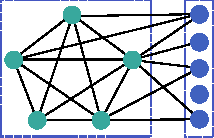
\includegraphics[scale=2]{pictures/(1_1)_graph.pdf}
    \caption{Grafo Split}
    \label{fig:split_1_1}
\end{figure}

\subsection{Reconhecimento de Grafos Split}

Sabemos que um grafo split é um grafo $\{C_4, C_5, 2K_2\}$-$free$, portanto, essas três propriedades classificamos como grafos proíbidos para a classe $split$, um algoritmo para reconhecimento dos grafos $split$ é verificar se o grafo $G$ é livre dessas três propriedades, caso a afirmação seja verdadeira, então o grafo é $split$.

\subsection{Grafos Cordais}

Dado um grafo $G = (V, E)$ é cordal quando o grafo possui todos os seus ciclos com pelo menos tamanho 4 que possuam uma corda em vértices não consecutivos com uma distância ímpar entre os vértices. Grafos cordais também são conhecidos como grafos $triangularizados$. Nas figuras \ref{fig:chordal_1} e \ref{fig:no_chordal} estão alguns exemplos de grafos cordal e não cordal, observamos que o grafo da figura \ref{fig:chordal_1} possui uma corda, que seria o vértice $\overline{ad}$ e o grafo não cordal da figura \ref{fig:no_chordal} não possui as arestas $\overline{ac}$ e $\overline{bd}$ no ciclo induzido $a, b, c, d, a$.

\begin{figure}
    \centering
    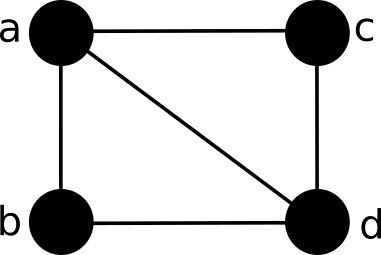
\includegraphics[scale=0.4]{pictures/path55.png}
    \caption{Grafo cordal}
    \label{fig:chordal_1}
\end{figure}

\begin{figure}
    \centering
    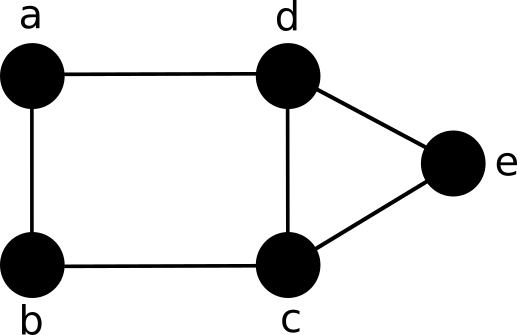
\includegraphics[scale=0.4]{pictures/non_chordal_1.png}
    \caption{Grafo não cordal}
    \label{fig:no_chordal}
\end{figure}

Os grafos cordais são uma subclasse dos grafos perfeitos. Um grafo é dito perfeito quando $\chi(G) = \omega(G)$.

Assim como os $grafos$-$(k,l)$, os grafos cordais também podem ser chamados de $(k,l)$-$cordais$ com a mesma propriedade do problema de particionamento, onde se quer particionar um grafo em $k$ conjuntos independentes e $l$ cliques. 


Há também a definição de grafo $cordal$-$(k,l)$, onde o grafo possui a mesma propriedade do problema de particionamento proposto por Brandstadt, de se particionar o grafo em $k$ conjuntos independentes e $l$ cliques, ou seja, é um $grafo$-$(k,l)$ e ser um grafo $cordal$.

A propriedade ser cordal é uma propriedade hereditária, portanto, qualquer subgrafo induzido de um grafo $cordal$ também será um grafo $cordal$.

\subsubsection{Reconhecimento de Grafos Cordais}

O reconhecimento dos grafos cordais pode ser feito através do algoritmo de busca lexicográfica ($LEX$-$BFS$). O $LEX$-$BFS$ é um algoritmo que se assemelha a busca em largura, porém com critérios de ordenação para exploração dos vértices de um grafo, maiores detalhes a respeito desse algoritmo podem ser conferidos no livro do Szwarcfiter \cite{JaymeGrafosNovo}.

\begin{lemma}
Seja $G = (V, E)$ um grafo cordal aplicado ao algoritmo de busca em largura lexicográfica. Então a sequência S de vértices $v$ ordenados decrescentemente segundo $largura(v)$ é um esquema de eliminação perfeita
\end{lemma}


O algoritmo de busca lexicográfica ($lex-BFS$) ordena todos os vértices do grafo em ordem descrecente, os grafos cordais possuem esquema de eliminação perfeita, portanto, executando o algoritmo $lex-BFS$ sobre um grafo cordal $G$, obtemos os vértices $\phi = v_1, v_2, ..., v_n$ em ordem descrescente, após obter a lista de vértices ordenada, deverá ser verificado se os vértices induzem uma clique, ou seja, se o vértice $v_i$ é simplicial, caso a afirmação seja verdadeira, então os vértices do conjunto retornado $\phi$ é um esquema de eliminação perfeita. Esse algoritmo de reconhecimento de grafos cordais possui a complexidade $O(nm)$.
